\documentclass{article}
\usepackage{graphicx} % Required for inserting images
\usepackage{geometry}

\newgeometry{vmargin={30mm}, hmargin={30mm,30mm}}   % set the margins

\title{Rapport DM 1}
\author{Grégoire DHIMOÏLA}
\date{April 2023}

\begin{document}

\maketitle

\section{Question 1}

$X$ is the set of black and white images of size 28x28 pixels. $Y$ is the set of labels $\{-1,1\}$ corresponding to the letter A or not.

\section{Question 2}

\subsection{}

The empirical risk is the average of the 0-1 loss over the training set. The true risk is the average over the whole input space following the distribution by which the training set is sampled. It is complicated to minimize the empirical risk because it is not differentiable and thus we cannot use gradient descent.

\subsection{}

We should use the test data to assess the performance because it is the only way to estimate the true risk of the predictor. Indeed, as we train only on the training set, there might be an overfitting problem, and the empirical risk might be very low, but the true risk might be high because the predictor is not general enough. So using the test data is the only way to estimate the true risk of the predictor.

\subsection{}
\begin{itemize}
    \item 
Linear least square regression:

minimize $1/n * \sum_{i=1}^n (f(X_i) - Y_i)^2$
\item 
Linear logistic regression:

minimize $1/n * \sum_{i=1}^n log(1 + e^{-Y_i f(X_i)})$
\end{itemize}

In both this problems, we consider $f$ as a linear function from $M_{28*28}(\mathbb{R})$ to $\mathbb{R}$. Thus, we can consider that we want to find an image of size 28*28 pixels, that will be used to compute the corellation between it and the input image.

My hypothesis at this point is that the resulting function image will resemble an A, and will probably be a somewhat average of the A images in the training set, maybe with mystical values in places where there might be confusion with B or C images. This would be the most satisfying result, but another possibility is that the resulting image will be composed of zeros everywhere except for a few high values where A images have almost always high values and not B and C, and highly negative values in the opposite situation. Thus the image might turn out to be black with a few bright spots.

\section{Question 3}

The code of this question can be found in the file \texttt{GradientDescent.py}.\newline

Comments on the code and results :\newline

All the results can be found in the results/GD file. The most interesting ones are synthesised here.

Due to the shear number of computations, the models could be trained on a CPU (arround 1-2 minutes for a GD with 10000 epochs), but I decided to accelerate this by using the GPU, which is much faster (arround 10 seconds for the same experiment). To do this, I used pytorch tensor instead of numpy arrays.

For the same amount of gradient steps, the model performs better with a bigger batch size, and takes only a little bit more time to train. This is thanks to the GPU acceleration of the torch engine.
This was to be expected as the GD gives a much more accurate direction for the gradient.
The figures below show the evolution of the loss and the accuracy over time for the different batch sizes.
See figure 1/2 for GD and SGD loss over gradient step. The final accuracy was 0.95 and 0.89 respectively.

The SGD produced images slightly noisier and the accuracy was much lower for the same amount of gradient steps (figures 3/4). Those images are really beautiful as they perfectly represent the expected result, with a clear positive A superposed to a clear neagative B/C, and neutral values on the intersection.\newline

We can see that when the prediction is kept as a real number, the model look like noise and performs slightly less than with a discrete predictions, where we take only the sign of the prediction (accuracy 0.95 vs 0.9).
This is coherent with the second hypothesis mentioned earlier, the model seems to concentrate on a few pixels and ignore the rest.
In the discrete case the model looks more like positive A and negative B/C shapes interlaced (See figures 4/5), which is coherent with the first hypothesis and to be honest, I expected this result everywhere...

The linear models performed slightly less than the logistic ones, and the main difference is in the image produced by the model. The logistic model produced clear images of the shapes and the linear produced really noisy images where the shape appeared only in the average over time (figure 4/6/7).

Another thing that seems to be of real help to the model is the normalization of the data. Indeed, the model performs much better with normalized data, and the images produced are slightly more coherent.
The convergence is a little bit slower but sometimes the raw cases simply diverged for some reason. The normalised ones were much more consistent.

\section{Question 4}

The code of this question can be found in the file \texttt{knn.py}.\newline

\subsection{}

The k-nearest neighbors classification rule with $L_2$ metric is the following :

for each test point, fint the k nearest neighbors in the training set, and predict the label of the test point as the most frequent label among the k neighbors.
We could also try to use a weighted vote, where the weight of each neighbor is inversely proportional to the distance to the test point.\newline

As a bonus, I also implemented le $K-means++$ algorithm, described below :

initialize the k cluster as points of the dataset chosen to maximize their mutual distance.
Then, for each point, assign it to the closest cluster, and update the cluster centers as the mean of the points assigned to it.
Repeat the last step until convergence.

To test the result, we compute the accuracy of the model on the test set.

\subsection{}

The results are in the results/knn folder (or figure 8) and are synthesised here.

The accuracy of the model stays arround 0.95 for k between 1 and 10. There is no clear tendency however in this range. As k increases, the error seems to increase too, wich is not verry suprising as, as already said, we are doing pixel-wise comparison, so allowing for more images, even if they are "close" also increases potential noise and confusion.

\subsection{}

The $K-folder$ cross validation is a method to estimate the performance of a model on a dataset. It consists in splitting the dataset in K parts, and for each part, train the model on the other parts and test it on the current part. Then, the performance is estimated as the average of the performance on each part.
In this case, it gives a best k of 3with a test accuracy of 0.94.

\subsection{Bonus : $K-means++$}

The results are in the results/kmeans folder (or figure 9/10/11) and are discussed here.\newline

My hypothesis for this algorithm was that it would already be pretty good for k = 2 as there are only two distinct class here (A and not A), but it would gain significantly in performance for k = 3 as there are three "real" class (A, B and C).
I figured that for k = 3 the performances would already be close to the maximum, and the clusters for 2 and 3 would resemble means of the letters.\newline

It so happens that even if the clusters are indeed averaged letters, the performance is really bad for k = 2, 3.
For k = 10, the performance is much more satisfying, but it is still not as good as the knn model.
It appears that the slight variations (in thickness or angle for example) found in the letters of the k=10 model are really important and explain why the k=2,3 models perform so badly. Indeed, the comparision between images is done pixel wise and thus is extremely not robust to small transformations of the images.

The difference in performance with knn is explained by the fact that knn is essentially a boosted version of K-means, where K = n. So it was to be expected that there would be a slight decrease in performance with regard to the knn model. However, the accuracy was still very impressive and could justify the abysal gain in computation.

\section{Question 5}

$$\begin{array}{|c|c|c|c|c|}
    \hline & \text { Logistic\ regression } & \text { Linear\ regression } & \text { K-NN } & \text { K-means }\\
    \hline \text { Empirical\ error\ (0-1\ loss) } & 0.096 & 0.026 & 0.18 & 0.091 \\
    \hline \text { Test error\ (0-1\ loss)} & 0.091 & 0.081 & 0.051 & 0.096 \\
    \hline
    \end{array}$$

\section{Figures}

\begin{figure}[h]
\centering
\includegraphics[width=0.8\textwidth]{GD_loss.png}
\caption{GD loss}
\end{figure}

\begin{figure}[h]
\centering
\includegraphics[width=0.8\textwidth]{SGD_loss.png}
\caption{SGD loss}
\end{figure}

\begin{figure}[h]
\centering
\includegraphics[width=0.8\textwidth]{SGD_model.png}
\caption{SGD model}
\end{figure}

\begin{figure}[h]
\centering
\includegraphics[width=0.8\textwidth]{GD_model.png}
\caption{GD model with discrete predictions}
\end{figure}

\begin{figure}[h]
\centering
\includegraphics[width=0.8\textwidth]{Continuous_model.png}
\caption{GD model with continuous predictions}
\end{figure}

\begin{figure}[h]
\centering
\includegraphics[width=0.8\textwidth]{Lin_model.png}
\caption{linear model}
\end{figure}

\begin{figure}[h]
\centering
\includegraphics[width=0.8\textwidth]{Lin_averages.png}
\caption{averaged linear model}
\end{figure}

\begin{figure}[h]
\centering
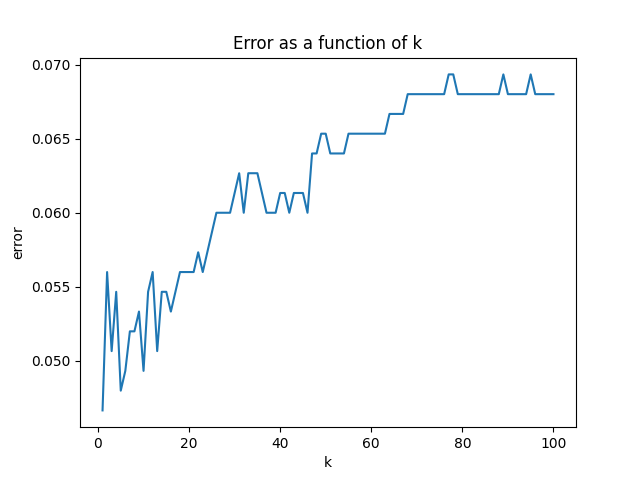
\includegraphics[width=0.8\textwidth]{knn_errors_1_100.png}
\caption{KNN errors}
\end{figure}

\begin{figure}[h]
\centering
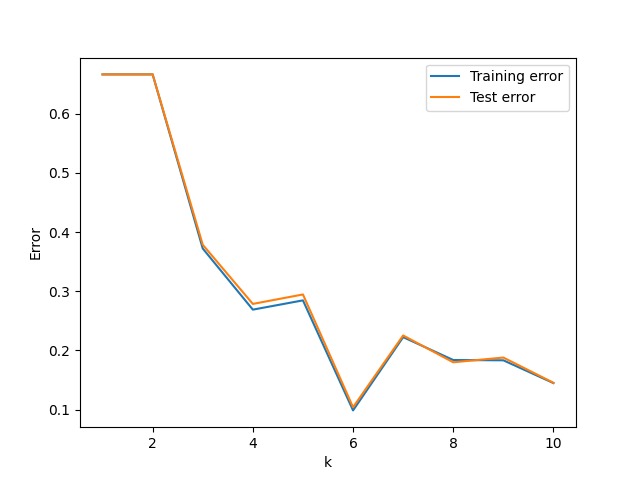
\includegraphics[width=0.8\textwidth]{kmeans.png}
\caption{kmeans}
\end{figure}

\begin{figure}[h]
\centering
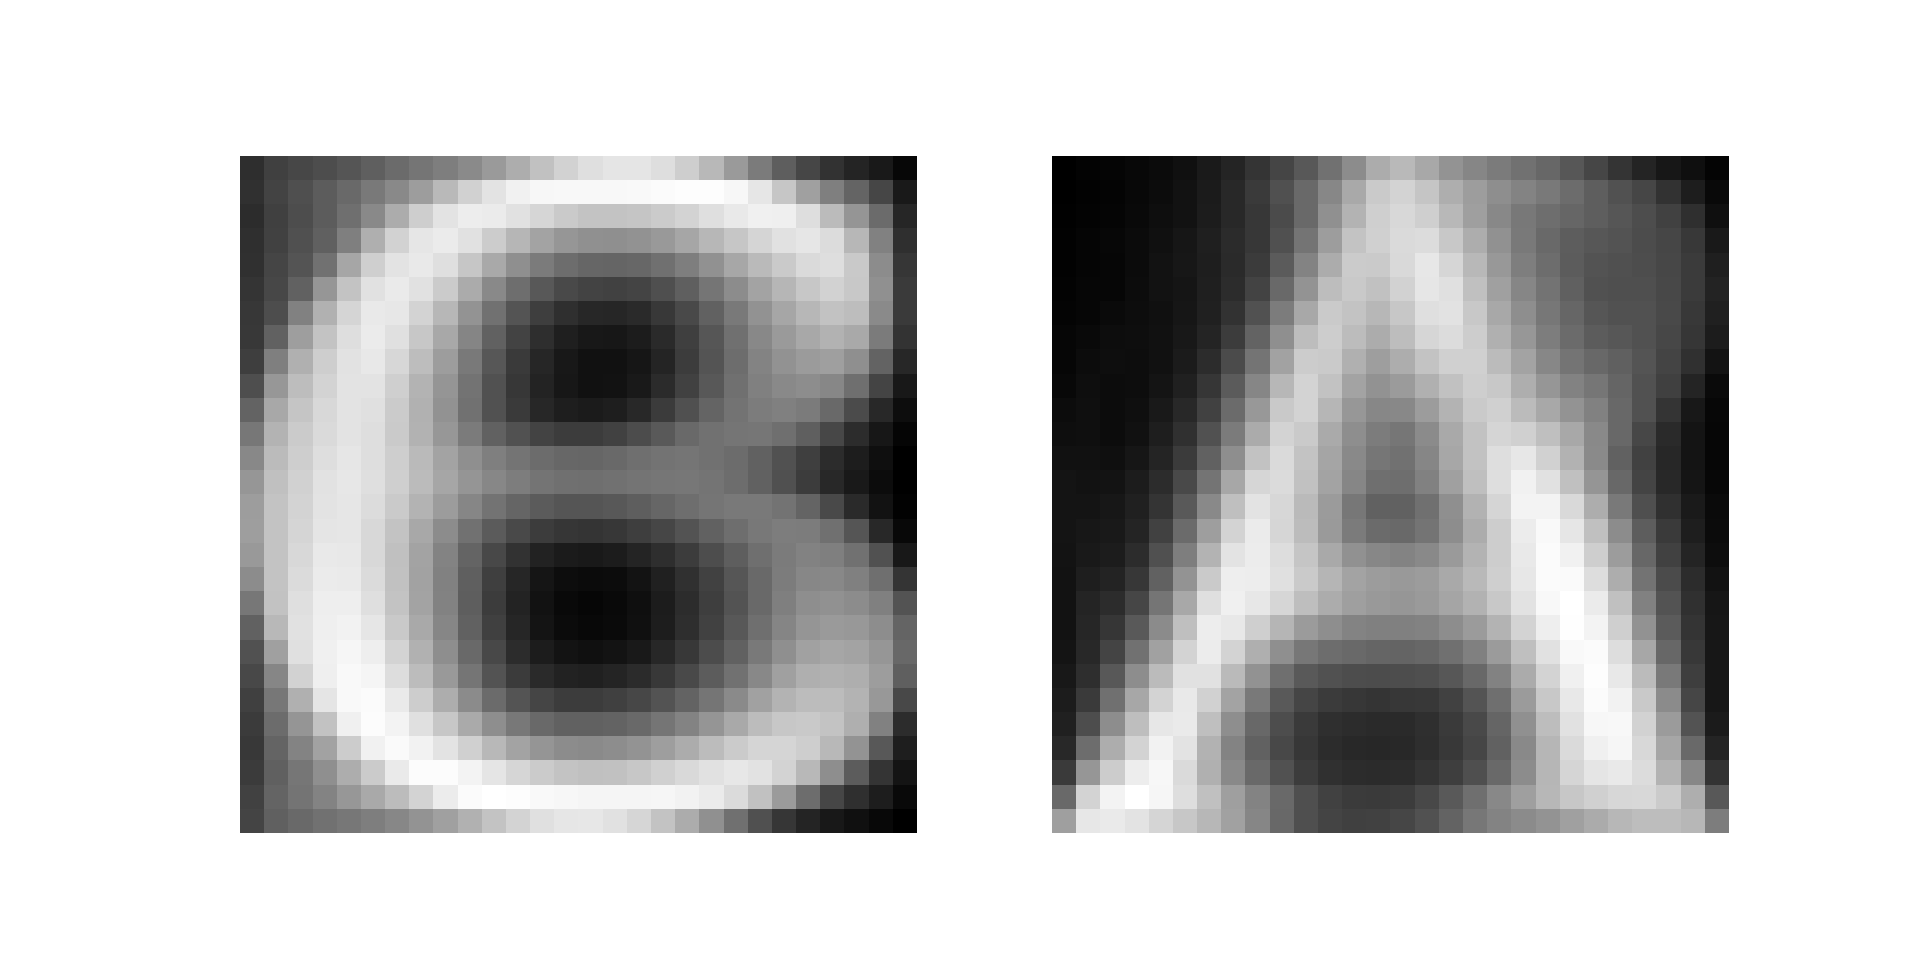
\includegraphics[width=0.8\textwidth]{kmeans_2.png}
\caption{kmeans, k = 2}
\end{figure}

\begin{figure}[h]
\centering
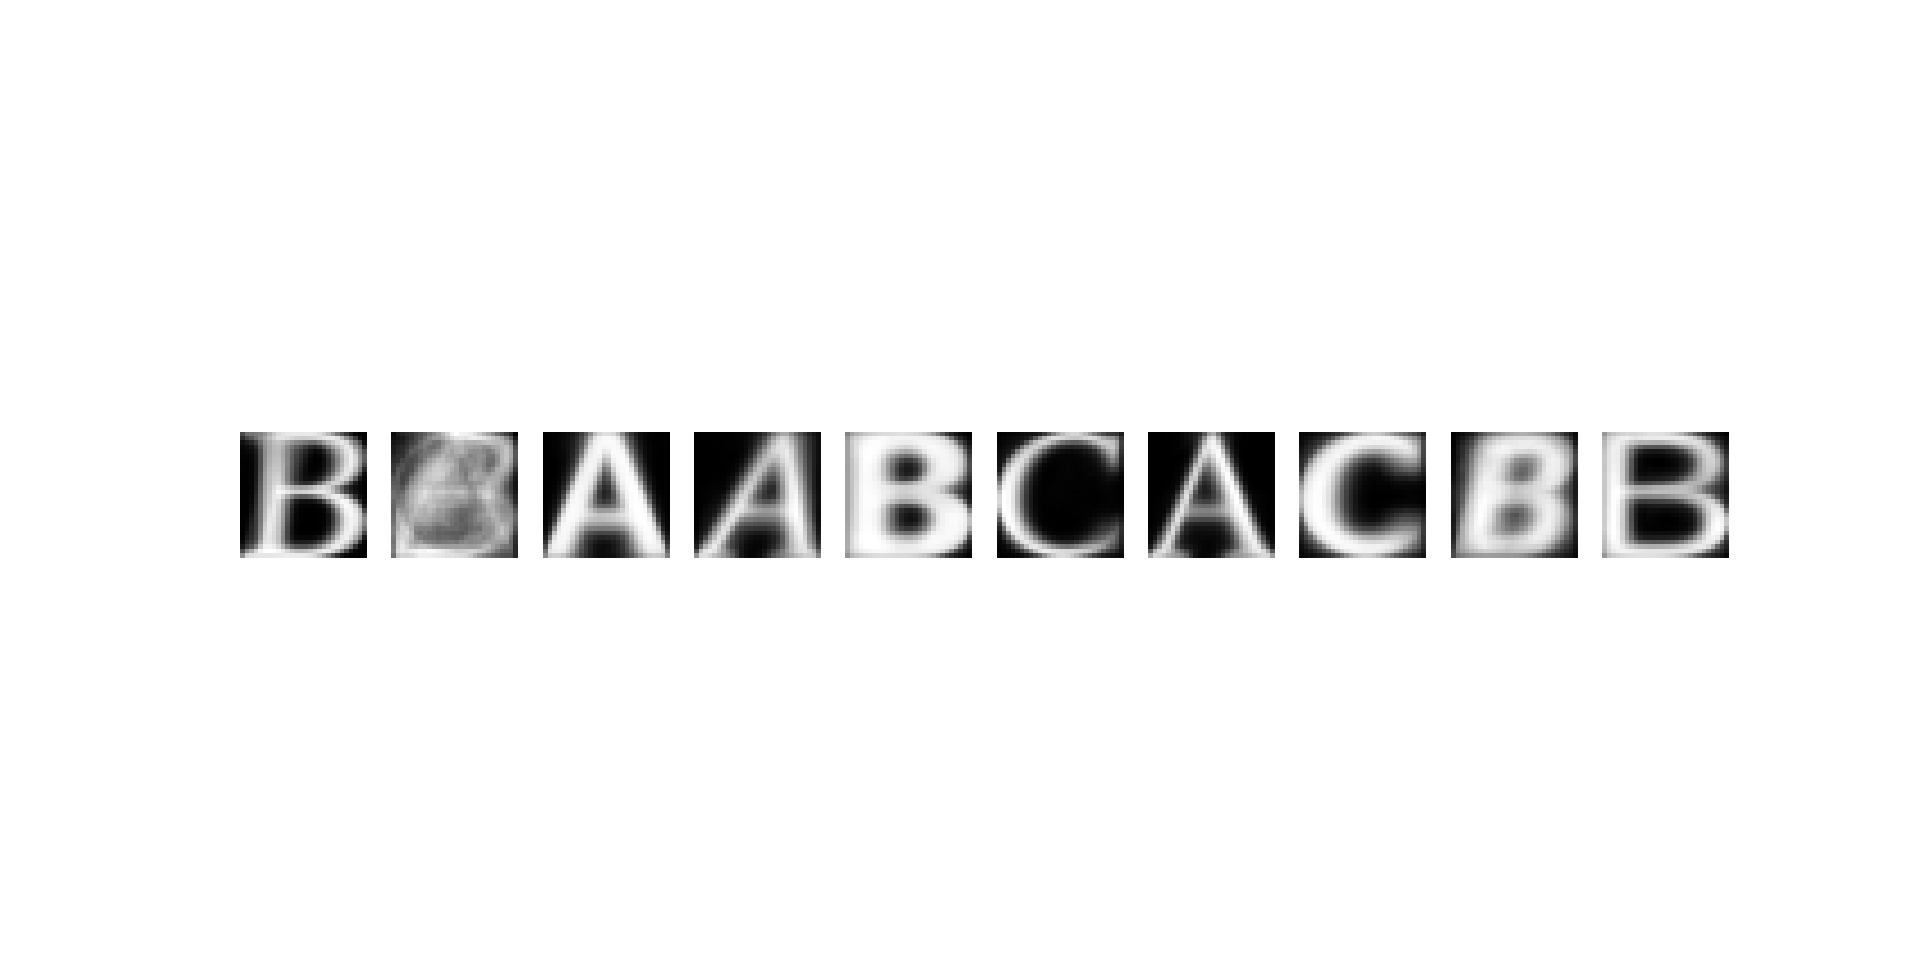
\includegraphics[width=0.8\textwidth]{kmeans_10.png}
\caption{kmeans, k = 10}
\end{figure}

\end{document}